%% =====================================================================
%%  Predicting Limit Order Books with Machine Learning -- Project Report
%%  Build:  ./build.sh        (runs pdflatex twice)
%%  Figures: python report/scripts/make_figures.py  (from the repo root)
%%  Edit the details in the block below, then rebuild.
%% =====================================================================
\newcommand{\ProjectTitle}{Predicting Limit Order Books with Machine Learning}
\newcommand{\ProjectSubtitle}{Accuracy, Speed and Cost: When Does a Price Prediction Pay?}
\newcommand{\CourseLine}{Machine Learning}            % <-- put the course code and name here
\newcommand{\GuideName}{[Guide Name]}                  % <-- put the guide's name here
\newcommand{\GuideDesignation}{[Designation]}          % <-- and the designation
\newcommand{\StudentOne}{1024030539 \quad Aarav Singhal}
\newcommand{\SubmissionMonth}{November 2026}
%% =====================================================================

\documentclass[12pt,a4paper,oneside]{report}
\usepackage[a4paper,left=3cm,right=2.5cm,top=2.5cm,bottom=2.5cm,headheight=15pt]{geometry}
\usepackage[T1]{fontenc}
\usepackage[utf8]{inputenc}
\usepackage{mathptmx}
\usepackage[scaled=0.82]{beramono}
\usepackage{amsmath,amssymb}
\usepackage{microtype}
\usepackage{setspace}
\usepackage{graphicx}
\usepackage{float}
\usepackage{caption}
\usepackage{subcaption}
\usepackage{booktabs}
\usepackage{tabularx}
\usepackage{longtable}
\usepackage{array}
\usepackage{enumitem}
\usepackage{xcolor}
\usepackage{colortbl}
\usepackage{listings}
\usepackage{titlesec}
\usepackage{fancyhdr}
\usepackage{tikz}
\usetikzlibrary{arrows.meta,positioning,shapes.geometric,calc,fit,backgrounds,decorations.pathreplacing}
\usepackage[hidelinks]{hyperref}

\onehalfspacing
\setlength{\parskip}{4pt}
\setlist{itemsep=2pt, topsep=4pt}
\captionsetup{font=small, labelfont=bf, skip=6pt}
\definecolor{tietblue}{gray}{0}
\definecolor{codebg}{gray}{0.96}
\definecolor{codeframe}{gray}{0.6}
\definecolor{rowgray}{gray}{0.93}
\definecolor{boxblue}{HTML}{DCEBF7}
\definecolor{boxorange}{HTML}{FBE5C8}
\definecolor{boxgreen}{HTML}{D5EFE3}
\definecolor{boxred}{HTML}{F6D5C9}
\definecolor{boxgrey}{gray}{0.92}

% ---------- chapter / section style ----------
\titleformat{\chapter}[display]
  {\normalfont\bfseries\color{tietblue}}
  {\large\MakeUppercase{\chaptertitlename}\ \thechapter}
  {6pt}{\LARGE}[\vspace{2pt}{\color{tietblue}\titlerule[1pt]}]
\titlespacing*{\chapter}{0pt}{-10pt}{18pt}
\titleformat{\section}{\normalfont\large\bfseries\color{tietblue}}{\thesection}{0.6em}{}
\titleformat{\subsection}{\normalfont\normalsize\bfseries}{\thesubsection}{0.6em}{}

% ---------- header / footer ----------
\pagestyle{fancy}
\fancyhf{}
\fancyfoot[C]{\small\thepage}
\renewcommand{\headrulewidth}{0pt}
\AddToHook{shipout/background}{\put(0,0){\tikz[overlay]\draw[line width=0.8pt]
  (1cm,-1cm) rectangle (\paperwidth-1cm,-\paperheight+1cm);}}
\fancypagestyle{plain}{\fancyhf{}\fancyfoot[C]{\small\thepage}\renewcommand{\headrulewidth}{0pt}}

% ---------- code listings ----------
\lstdefinestyle{py}{
  language=Python, basicstyle=\ttfamily\scriptsize, keywordstyle=\bfseries,
  commentstyle=\color{gray}\itshape, backgroundcolor=\color{codebg},
  frame=single, rulecolor=\color{codeframe}, numbers=left, numberstyle=\tiny\color{gray},
  numbersep=6pt, xleftmargin=1.6em, framexleftmargin=1.4em, breaklines=true,
  showstringspaces=false, tabsize=4, columns=fullflexible, keepspaces=true,
  aboveskip=6pt, belowskip=6pt, captionpos=b}
\lstdefinestyle{console}{
  language={}, numbers=none, basicstyle=\ttfamily\scriptsize, backgroundcolor=\color{codebg},
  frame=single, rulecolor=\color{codeframe}, breaklines=true, columns=fixed,
  keepspaces=true, showstringspaces=false, xleftmargin=0pt, aboveskip=6pt, belowskip=6pt, captionpos=b}
\lstset{style=py}
\renewcommand{\lstlistingname}{Listing}

\newcommand{\code}[1]{\texttt{#1}}
\newcommand{\bp}{\,bp}
\sloppy
\setlength{\emergencystretch}{3em}
\newcommand{\fig}[3]{%
  \begin{figure}[H]\centering
  \includegraphics[width=#2\linewidth]{figures/#1}
  \caption{#3}\label{fig:#1}\end{figure}}

\hypersetup{pdftitle={Predicting Limit Order Books with Machine Learning -- Project Report},
            pdfauthor={Aarav Singhal}}

\begin{document}

%% =====================================================================
%%  COVER PAGE
%% =====================================================================
\begin{titlepage}
\thispagestyle{empty}
\centering\singlespacing
\vspace*{0cm}
{\Large\bfseries \CourseLine\par}
\vspace{0.4cm}
{\large Project Report\par}
\vspace{0.45cm}
{\color{tietblue}\rule{\linewidth}{1.2pt}\par}
\vspace{0.35cm}
{\huge\bfseries\color{tietblue} \ProjectTitle\par}
\vspace{0.3cm}
{\large\itshape \ProjectSubtitle\par}
\vspace{0.25cm}
{\color{tietblue}\rule{\linewidth}{1.2pt}\par}
\vspace{0.45cm}
{\large Under the Guidance of\par}
\vspace{0.4cm}
{\Large\bfseries \GuideName\par}
\vspace{0.1cm}
{\large \GuideDesignation\par}
{\large Thapar Institute of Engineering \& Technology\par}
\vspace{0.35cm}

\includegraphics[height=2.4cm]{figures/thapar_logo.png}\par
\vspace{0.3cm}
\begin{flushleft}
{\large\bfseries Submitted By:\par}
\vspace{0.25cm}
{\large \StudentOne\par}
\end{flushleft}
\vfill
{\large Computer Science \& Engineering Department\par}
{\large Thapar Institute of Engineering \& Technology, Patiala\par}
\vspace{0.35cm}
{\normalsize In Partial Fulfilment of the Requirements for the Degree of\par}
{\normalsize\bfseries Bachelor of Engineering in Computer Engineering\par}
\vspace{0.2cm}
{\normalsize at\par}
\vspace{0.2cm}
{\normalsize Thapar Institute of Engineering \& Technology, Patiala\par}
\vspace{0.35cm}
{\large\bfseries \SubmissionMonth\par}
\end{titlepage}

%% =====================================================================
%%  FRONT MATTER
%% =====================================================================
\pagenumbering{roman}
\setcounter{page}{1}

\chapter*{Abstract}
\addcontentsline{toc}{chapter}{Abstract}

Most machine-learning work on financial prices uses bars: one open, high, low and close price per minute or per day. A \textbf{limit order book (LOB)} is much richer. It lists every resting buy and sell order at every price, updates many times a second, and shows the supply and demand that will move the price \emph{before} it moves. This project asks two connected questions. First, \emph{how much can machine learning predict} about the next few seconds of price movement from LOB data, which models do it best, and are the gains statistically real? Second, \emph{does a correct prediction actually make money} once a trading system has to act on it, which depends on how accurate the model is, how fast it runs, and what each trade costs?

Data were collected from five real sources (one-second Coinbase BTC-USD and ETH-USD books, about 1.03 million snapshots each; every order event for five Nasdaq stocks from LOBSTER; the FI-2010 academic benchmark; and two public volatility and auction datasets) and a synthetic order book with a planted signal. All books were converted to one 40-column format, labelled, and split chronologically with purging so that no future information reaches the training data. Twenty-seven causal microstructure features (order flow imbalance, multi-level OFI with PCA, VPIN, micro-price, queue imbalances, book slopes and lags) feed the tabular models, and raw $100\times40$ book windows feed the deep models, which were trained on Google Colab A100 GPUs. The model ladder runs from naive baselines through logistic regression, Random Forest and LightGBM to an LSTM, DeepLOB (CNN + Inception + LSTM) and a transformer (TLOB). Tasks include three-class classification (UP/FLAT/DOWN), regression of future price changes and volatility, and binary classification of toxic fills.

\begin{itemize}[leftmargin=1.5em, itemsep=1pt, topsep=3pt]
  \item \textbf{The book is predictive, but modestly.} On BTC at 20\,s, LightGBM reaches macro-F1 0.467 (random 0.333, momentum 0.413) and a one-vs-rest ROC-AUC of about 0.66. It beats every other model with block-bootstrap confidence intervals that exclude zero. On large-tick Nasdaq stocks the signal is stronger and peaks 1--5\,s ahead.
  \item \textbf{Simpler models beat deep networks at short horizons, in accuracy as well as speed.} On BTC at 20\,s, LightGBM is more accurate than DeepLOB (accuracy 0.476 vs 0.429, macro-F1 0.467 vs 0.401), the LSTM and TLOB. On FI-2010, logistic regression with book history beats our DeepLOB at $k=10$ (86.1\% vs 83.1\%). DeepLOB wins only at longer horizons ($k=50$--100). Our DeepLOB reproduces the published paper to within 0.7--2.3 points.
  \item \textbf{Speed matters, but only relative to cost and signal decay.} On a synthetic book, both models lose about \$4 of profit per millisecond of latency, so DeepLOB's extra 2.3\,ms costs about \$10, while LightGBM's better signal is worth \$350: accuracy is worth 35 times more than inference speed there. The more accurate model also stays profitable up to $>$100\,ms, while DeepLOB's profit is gone by about 29\,ms. On BTC, the best signals earn 2.2\bp\ before costs and the most confident ones lose three times as much to a one-second delay, but a round trip costs 8\bp\ in fees alone, so no model can pay.
  \item \textbf{The fastest accurate model wins.} LightGBM compiled to C++ reproduces the Python model exactly and predicts in 10.5\,$\mu$s, 230--540 times faster than DeepLOB on a GPU, while being more accurate on BTC.
\end{itemize}

The conclusion is a rule for using LOB machine learning: trading costs set the bar, accuracy decides whether a model clears it, and latency matters in proportion to how quickly the signal decays.

\vspace{0.4cm}
\noindent\textbf{Keywords:} limit order book, high-frequency data, market microstructure, gradient boosting, LightGBM, DeepLOB, transformer, order flow imbalance, data leakage, purged cross-validation, inference latency, transaction costs.

\tableofcontents
\listoffigures
\listoftables

\clearpage
\pagenumbering{arabic}
\setcounter{page}{1}

%% =====================================================================
%%  CHAPTER 1  INTRODUCTION
%% =====================================================================
\chapter{Introduction}

\section{Background: what a limit order book is}

On almost every modern exchange (stocks, futures, cryptocurrencies) trading happens through a \textbf{limit order book}. A trader who wants to buy can post a \emph{limit order}: ``I will buy 2 BTC at \$56{,}000 or less''. That order rests in the book until someone sells to it or it is cancelled. All resting buy orders form the \textbf{bid} side and all resting sell orders the \textbf{ask} side (Figure~\ref{fig:btc_book_snapshot}). The highest bid and the lowest ask are the \emph{best quotes}; the gap between them is the \textbf{spread}, and their average is the \textbf{mid price}. A trader who wants to trade immediately sends a \emph{market order}, which ``crosses the spread'' and fills against the resting orders on the other side, walking through levels if it is large.

\fig{btc_book_snapshot}{1.0}{The raw material of the project. Left: one second of the Coinbase BTC-USD book, with the resting size at each of the first 10 price levels on each side. Right: one hour of the mid price and the 10th level on each side.}

The book changes every time an order arrives, trades or is cancelled, which on a busy market is thousands of times per second. Each snapshot is a $10\text{ levels}\times 4$ (ask price, ask size, bid price, bid size) $=40$-number picture of supply and demand.

\section{Why LOB data is a novel input for machine learning}\label{sec:novelty}

Most machine-learning projects on prices use \emph{bars}: one open/high/low/close/volume (OHLCV) record per minute or per day. Bars only record the prices at which trades happened. They do not record the \emph{orders waiting to trade}, which is where the pressure that moves the next price shows up. Table~\ref{tab:novelty} compares the two kinds of data.

\begin{table}[H]
\centering\small
\caption{OHLCV bar data compared with limit order book data}
\label{tab:novelty}
\begin{tabularx}{\linewidth}{@{}>{\raggedright\arraybackslash}p{3.2cm}>{\raggedright\arraybackslash}X>{\raggedright\arraybackslash}X@{}}
\toprule
 & \textbf{OHLCV bars} & \textbf{Limit order book (this project)} \\
\midrule
What is recorded & Prices of completed trades, summarised per bar & Every resting order at 10 levels per side, plus each add, trade and cancel \\
Time resolution & Minutes to days & 100\,ms (Nasdaq) to 1\,s (BTC); events are microseconds apart \\
Rows per day & 390 (1-minute bars, stock) & 86{,}400 (BTC, 1\,s) to 234{,}000 (Nasdaq, 100\,ms) \\
Values per row & 5 & 40 raw values, plus order flows \\
Shows supply/demand before the price moves & No & Yes: queue sizes, imbalance, cancellations \\
Main ML difficulty & Very low signal-to-noise & Huge, autocorrelated, non-stationary data; leakage; tiny moves relative to costs \\
Who can trade on the prediction & Anyone, slowly & Only a system fast enough to act within seconds \\
\bottomrule
\end{tabularx}
\end{table}

The extra information is real. Figure~\ref{fig:btc_imbalance_signal} sorts every BTC snapshot by its \emph{queue imbalance} (how much more size waits on the bid than on the ask) and plots the average price change over the next 20 seconds. The relation is monotone: when the book leans towards the bid, the price tends to rise, and vice versa. No bar dataset contains this variable. The difficulty, and what the rest of the report is about, is that the effect is a fraction of a basis point (1\bp\ $=0.01\%$), so the question is not only whether a model can learn it, but whether anyone could trade on it.

\fig{btc_imbalance_signal}{1.0}{Evidence that the book carries information about the next price move (BTC, all 1.03 million snapshots). Left and centre: mean 20\,s mid-price change by decile of level-1 and 10-level queue imbalance, with 95\% confidence intervals. Right: the distribution of 20\,s moves is sharply peaked at zero and heavy-tailed.}

\section{Problem statement}

Published deep-learning papers report 80\%+ accuracy at predicting short-term mid-price moves from LOB data. These numbers raise three questions that this project answers with experiments:
\begin{enumerate}
  \item \textbf{Is the predictability real?} High-frequency data make it easy to leak future information into training (overlapping labels, normalising with full-sample statistics, shuffled cross-validation), and accuracy is misleading when most moves are ``flat''. Which models genuinely beat simple baselines on held-out future data, and by a statistically significant margin?
  \item \textbf{Which models, and why?} Do deep networks that read the raw book (DeepLOB, transformers) beat gradient-boosted trees on hand-crafted microstructure features? Which parts of the book carry the signal, and for how long does it last?
  \item \textbf{Does accuracy become profit?} A prediction is only valuable if a trading system can act on it before it expires and after paying the spread and fees. How do model accuracy, model \emph{speed} (inference latency) and trading cost combine to decide whether a model makes money?
\end{enumerate}

\section{Objectives}

\begin{enumerate}
  \item Collect and clean LOB data from several real markets with different properties (crypto vs stocks, small vs large tick size), and convert them to one common format.
  \item Engineer causal microstructure features from the literature (OFI, multi-level OFI with PCA, VPIN, micro-price, imbalance, book slope) with all fitted transforms estimated on training data only.
  \item Build a leakage-controlled evaluation: chronological purged splits, train-only label thresholds, identical test rows for every model, negative controls, and significance tests suitable for autocorrelated data.
  \item Train and compare a ladder of models: naive baselines, logistic regression, Random Forest, LightGBM, LSTM, DeepLOB and TLOB, on classification and regression tasks, and report accuracy, macro-F1, ROC-AUC, log-loss, MCC, information coefficient, $R^2$ and other measures.
  \item Measure how fast the predictive signal decays with horizon and which features the models rely on (ablation, TreeSHAP, gradient attribution).
  \item Build an execution simulator (spread crossing, book walking, fees, latency, passive fills) and measure each model's inference latency, including a C++ version of the trained model, to quantify how accuracy and speed together decide profit.
\end{enumerate}

\section{Contributions}

\begin{itemize}
  \item A single, tested pipeline (40 automated tests) that runs the same features, models and evaluation on synthetic data, Coinbase BTC-USD, Nasdaq LOBSTER and FI-2010.
  \item A fair model comparison on BTC with block-bootstrap confidence intervals and McNemar tests, showing that LightGBM is significantly better than every baseline and than DeepLOB.
  \item A reproduction of the published DeepLOB result on FI-2010, and evidence that its short-horizon advantage comes from seeing book \emph{history}, not from its architecture.
  \item A decomposition of the trading edge into accuracy, latency and cost components, a break-even accuracy formula, and a latency sweep that converts milliseconds into dollars.
  \item A code generator that compiles the trained LightGBM model into plain C++ with bit-identical output and microsecond inference.
\end{itemize}

\section{Organisation of the report}

Chapter~2 reviews the relevant literature. Chapter~3 describes how the data were collected, explored and preprocessed. Chapter~4 covers feature engineering. Chapter~5 describes the learning tasks, the models and the validation method. Chapter~6 presents the prediction results, and Chapter~7 links accuracy and speed to profit. Chapter~8 discusses limitations and future work, and Chapter~9 concludes.

%% =====================================================================
%%  CHAPTER 2  LITERATURE REVIEW
%% =====================================================================
\chapter{Literature Review}

\section{Microstructure signals}

\paragraph{Order flow imbalance (OFI).} Cont, Kukanov and Stoikov~\cite{cont2014} showed that short-term price changes are explained, almost linearly, by the net change in supply and demand at the best quotes: new bids and cancelled asks push the price up, and the reverse pushes it down. Their OFI variable counts these changes from one snapshot to the next. Multi-level OFI extends it to deeper levels.

\paragraph{Queue imbalance and the micro-price.} When the bid queue is much larger than the ask queue, the ask is more likely to be depleted first, so the next mid-price move is more likely up. Stoikov~\cite{stoikov2018} formalised this as the \emph{micro-price}, an estimator of the ``fair'' price that weights each best quote by the size on the opposite side.

\paragraph{Flow toxicity (VPIN).} Easley, L\'opez de Prado and O'Hara~\cite{easley2012} proposed VPIN, the volume-synchronised probability of informed trading, as a measure of how one-sided recent trading has been. High VPIN was argued to signal ``toxic'' flow that hurts market makers.

\section{Machine learning on limit order books}

\begin{table}[H]
\centering\small
\caption{Key prior work used or tested in this project}
\label{tab:lit}
\begin{tabularx}{\linewidth}{@{}>{\raggedright\arraybackslash}p{3.6cm}>{\raggedright\arraybackslash}X>{\raggedright\arraybackslash}p{4.0cm}@{}}
\toprule
\textbf{Work} & \textbf{Contribution} & \textbf{Used here as} \\
\midrule
Ntakaris et al.\ 2018~\cite{ntakaris2018} & FI-2010, the first public LOB benchmark (5 Finnish stocks, 10 days, 144 features) & Benchmark dataset \\
Zhang, Zohren, Roberts 2019~\cite{zhang2019} (DeepLOB) & CNN + Inception + LSTM on raw $100\times40$ book windows; 84.5\% accuracy on FI-2010 & Tier-5 model, reproduced \\
Tran et al.\ 2021~\cite{tran2021} & Bilinear normalisation (BiN) for non-stationary LOB series & Inside TLOB \\
Berti, Kasneci 2025~\cite{berti2025} (TLOB) & Transformer with attention over time and features & Tier-5 model (simplified) \\
Cont et al.\ 2014~\cite{cont2014} & Order flow imbalance & Features \\
Easley et al.\ 2012~\cite{easley2012} & VPIN & Feature and regime variable \\
Stoikov 2018~\cite{stoikov2018} & Micro-price & Feature, predictor and target \\
Ke et al.\ 2017~\cite{ke2017} (LightGBM) & Histogram-based, leaf-wise gradient boosting & Tier-3 model \\
L\'opez de Prado 2018~\cite{lopez2018} & Purged and embargoed cross-validation for financial ML & Validation design \\
Lundberg, Lee 2017~\cite{lundberg2017} (SHAP) & Additive feature attribution; TreeSHAP & Model explanation \\
\bottomrule
\end{tabularx}
\end{table}

\section{Gaps this project addresses}

\begin{enumerate}
  \item \textbf{Accuracy without costs.} Most LOB papers stop at classification accuracy. Profit at the mid price with no fees, which several report, is not achievable by a real trader. This project carries predictions through an execution simulator.
  \item \textbf{Smoothed labels and a single dataset.} FI-2010 labels average future prices, which makes them easier to predict, and FI-2010 is one market in 2010. This project tests the same models on crypto and on Nasdaq data with different tick sizes.
  \item \textbf{Speed treated separately from accuracy.} Deep models are slower; whether that matters depends on how quickly the signal decays. This project measures both and converts latency into lost profit.
\end{enumerate}

%% =====================================================================
%%  CHAPTER 3  DATA
%% =====================================================================
\chapter{Data Collection and Preprocessing}

\section{Data sources}

Six datasets were used. Each has a specific job in the project (Table~\ref{tab:data}).

\begin{table}[H]
\centering\small
\caption{Datasets, their size and their role}
\label{tab:data}
\begin{tabularx}{\linewidth}{@{}>{\raggedright\arraybackslash}p{2.7cm}>{\raggedright\arraybackslash}X>{\raggedright\arraybackslash}p{3.3cm}>{\raggedright\arraybackslash}p{3.3cm}@{}}
\toprule
\textbf{Dataset} & \textbf{Content and source} & \textbf{Size used} & \textbf{Role} \\
\midrule
Coinbase BTC-USD & 15-level book snapshot every second, trade volumes, per-level add/trade/cancel flows. Public CC0 dataset recorded from Coinbase & 1.03 million snapshots, 7--19 April 2021 (12 days), split into 4 segments of $\approx$3 days & Main real testbed: models, horizons, attribution, execution \\
Coinbase ETH-USD & Same format and dates & 1.03 million snapshots & Cross-asset features \\
LOBSTER (Nasdaq) & Every order event (add, cancel, execute) and the 10-level book after it, for INTC, MSFT, AAPL, AMZN, GOOG. Free academic samples from lobsterdata.com~\cite{huang2015} & One full day (21 June 2012, 9:30--16:00) per stock, resampled to 100\,ms ($\approx$234{,}000 rows each) & Sub-second horizons; large- vs small-tick stocks; market making \\
FI-2010 & 5 Finnish stocks on Nasdaq Nordic, 10 days in June 2010, already normalised, 144 features and labels & Setup 2: train days 1--7, test days 8--10 & Comparison with published DeepLOB \\
Realised volatility (Optiver) & Two-level book and trades per second in 10-minute windows, $\approx$112 stocks & Full training set, 4 forward folds & Regression; leakage case study \\
Closing auction (Optiver) & Nasdaq closing-auction imbalance for 200 stocks & 481 days, 5.2 million rows & Regression under drift \\
Synthetic & Simulated 10-level book with a planted ``informed trader'' & 5 sessions $\times$ 60{,}000 events & Controlled tests; latency sweep \\
\bottomrule
\end{tabularx}
\end{table}

\paragraph{Tick size.} The \emph{tick} is the smallest allowed price step. It shapes everything that follows. INTC and MSFT are \textbf{large-tick} stocks: one cent is 3.3--3.7\bp\ of their price, the spread is one tick 77\% of the time, and about 13{,}000 shares wait at the best price. AAPL, AMZN and GOOG are \textbf{small-tick} (0.17--0.45\bp), with about 100 shares at the best price. BTC is extremely small-tick: \$0.01 on a price of about \$60{,}000 is 0.0017\bp.

\section{How the data were collected}

\begin{itemize}
  \item \textbf{Crypto (BTC, ETH).} Downloaded programmatically with the Kaggle API by \code{scripts/fetch\_datasets.py}, which reads credentials from the environment (or Colab secrets) and is cross-platform. The raw CSVs are 1.8\,GB per coin.
  \item \textbf{LOBSTER.} The free academic sample files (message file + order-book file per stock) were downloaded manually from lobsterdata.com and unzipped into \code{data/raw/lobster/}. They cannot be redistributed, so they are not in the repository.
  \item \textbf{FI-2010 and the two volatility/auction datasets.} Downloaded with the same fetcher; the competition data require accepting the data rules once.
  \item \textbf{Synthetic data.} Generated on the fly by \code{src/data/synthetic\_generator.py}: a 10-level book with a \$100 price and 1-cent tick, events every $\approx$10\,ms (40\% market orders, 40\% limit orders, 20\% cancellations). An ``informed trader'' switches on for 15--60 events at random, sending 85\% of market orders one way and tilting limit orders and cancellations, so the book leans before the price moves.
\end{itemize}

\paragraph{Compute.} Feature extraction, tabular models and simulations ran on a laptop CPU (12 cores, 14\,GB RAM). All deep-learning training (LSTM, DeepLOB and TLOB on BTC, the synthetic book and FI-2010) was done on \textbf{NVIDIA A100 GPUs on Google Colab}, Google's cloud notebook service; a full BTC run of the three deep models took a few hours, and DeepLOB alone about 18 minutes per segment. Every long experiment checkpoints after each segment or horizon, and \code{scripts/sync\_checkpoints.py} pushes the checkpoints to a git branch so that a run interrupted on one machine can continue on the other.

\section{A common representation}

Every book dataset is converted into the same layout so that one feature pipeline and one set of models work on all of them. One snapshot is a row of 40 numbers:
\[
\mathbf{x}_t = \big[p^a_1, q^a_1, p^b_1, q^b_1,\; p^a_2, q^a_2, p^b_2, q^b_2,\; \dots,\; p^a_{10}, q^a_{10}, p^b_{10}, q^b_{10}\big],
\]
where $p^a_m, q^a_m$ are the price and size of the $m$-th ask level and $p^b_m, q^b_m$ the same for the bid. Alongside it each dataset provides millisecond timestamps and a trade tape (time, price, size, buy/sell side) for VPIN and the execution simulator.

\section{Exploratory data analysis}

Table~\ref{tab:eda} summarises the properties that most affect learning.

\begin{table}[H]
\centering\small
\caption{Properties of the real order-book data}
\label{tab:eda}
\begin{tabular}{@{}lccc@{}}
\toprule
 & \textbf{BTC-USD} & \textbf{INTC, MSFT} & \textbf{AAPL, AMZN, GOOG} \\
\midrule
Clock & 1\,s & 100\,ms & 100\,ms \\
Tick as share of price & 0.0017\bp & 3.3--3.7\bp & 0.17--0.45\bp \\
Spread at one tick & 80\% & 77\% & under 1\% \\
Typical size at best price & a few BTC & $\approx$13{,}000 shares & $\approx$100 shares \\
Mid changes per minute & -- & 8--10 & 60--165 \\
Mean $|$20\,s move$|$ & 3.3\bp & -- & -- \\
Correlation(L1 imbalance, next move) & 0.14 (20\,s) & 0.24 (INTC, 5\,s) & 0.04 (AMZN, 5\,s) \\
\bottomrule
\end{tabular}
\end{table}

Three observations from this analysis shaped the method:
\begin{enumerate}
  \item \textbf{Most moves are tiny.} 59\% of one-second BTC mid changes are exactly zero, and the 20\,s distribution is sharply peaked and heavy-tailed (Figure~\ref{fig:btc_imbalance_signal}, right). Labels therefore need a threshold, and accuracy alone is a misleading metric.
  \item \textbf{The book is informative, and more so for large ticks.} Figure~\ref{fig:lobster_imbalance_signal} repeats the imbalance analysis on Nasdaq. On the large-tick INTC the 5\,s move rises steeply with queue imbalance; on the small-tick AMZN the relation is much weaker, because its queues are small and change constantly.
  \item \textbf{The data are non-stationary.} Volatility and volume differ strongly between days. This is why every BTC experiment is repeated on four separate segments, and why FI-2010's calmer test days later cause a measurable distribution shift.
\end{enumerate}

\fig{lobster_imbalance_signal}{0.95}{Queue imbalance against the next 5\,s mid change on Nasdaq (100\,ms clock, whole day). The large-tick stock (left) shows a strong, monotone relation; the small-tick stock (right) a weak one.}

\section{Preprocessing}

\subsection{Conversion and cleaning}
\begin{itemize}
  \item \textbf{BTC/ETH.} The raw file stores each level as a \emph{distance from the mid} and a \emph{USD notional}. Prices are rebuilt as $\text{mid}\times(1+\text{distance})$ and rounded to the 1-cent tick; sizes are notional/price in BTC. The first 10 of 15 levels are kept. A trade tape is rebuilt from the per-second buy and sell volumes. The result is cached as a compressed NumPy file (370\,MB) so later runs load in seconds.
  \item \textbf{LOBSTER.} Prices are stored as dollars $\times$ 10{,}000 and converted. Empty levels (marked with dummy prices) are set to missing. The event stream is \textbf{resampled onto a 100\,ms clock}: each row is the book as it stood at that instant (last event at or before it), so horizons such as 500\,ms or 5\,s become a fixed number of rows. Executions between rows become the trade tape, and adds, trades and cancels per level become order-flow features.
  \item \textbf{FI-2010.} The files store features as rows and time as columns, so they are transposed; the five label rows (horizons 10, 20, 30, 50, 100 events) are separated from the 144 features.
  \item \textbf{Missing and padded values.} Zero or NaN-padded levels are handled explicitly in the simulator; any remaining NaN or infinite feature values (for example a ratio with zero depth) are set to 0 after feature computation.
\end{itemize}

\subsection{Segmentation}
The 1.03 million BTC rows are cut into \textbf{four contiguous segments of 257{,}682 rows} ($\approx$3 days each). Each segment is treated as an independent repetition of the whole experiment, with its own train/validation/test split, label thresholds, feature fitting and VPIN bucket size. Results are reported as mean $\pm$ standard deviation over the four segments. Synthetic results use five independently generated seeds.

\subsection{Label construction}
For a horizon of $k$ rows, the label compares a smoothed future mid price with the current one:
\[
r_t = \frac{\bar m_{t+k} - m_t}{m_t}, \qquad
y_t = \begin{cases} \text{UP} & r_t > \theta \\ \text{DOWN} & r_t < -\theta \\ \text{FLAT} & \text{otherwise}\end{cases}
\]
where $\bar m$ is a 5-row trailing mean of the mid. On synthetic data $\theta = 1.5$\bp. On BTC, $\theta$ is chosen \textbf{on the training rows only} so that one third of training labels are FLAT, which puts random guessing at macro-F1 $\approx 0.333$ and makes the three classes comparably important. LOBSTER uses unsmoothed labels; FI-2010 uses its own published labels (mean of the next $k$ mids, $\pm0.2\%$).

Some experiments use other targets: the future mid change in basis points (regression, Section~\ref{sec:regression}), a \emph{cost-aware} label that is UP only if buying at the ask and selling at the bid $k$ seconds later beats the fees, and a binary ``toxic fill'' label for market making.

\paragraph{Class balance.} The share of FLAT labels depends strongly on the horizon and the market (Table~\ref{tab:flat}). At short horizons on large-tick stocks almost every label is FLAT, so a model that always says FLAT has very high accuracy and no use. This is why macro-F1, which weights the three classes equally, is the main metric, and why every learned model uses balanced class weights.

\begin{table}[H]
\centering\small
\caption{Share of FLAT labels in the test period}
\label{tab:flat}
\begin{tabular}{@{}lcccccc@{}}
\toprule
\textbf{Data} & \multicolumn{6}{c}{\textbf{Horizon}} \\
\midrule
Nasdaq (100\,ms clock) & 100\,ms & 500\,ms & 1\,s & 5\,s & 10\,s & 30\,s \\
\quad INTC (large tick) & 99\% & 97\% & 95\% & 80\% & 66\% & 42\% \\
\quad MSFT (large tick) & 99\% & 96\% & 93\% & 74\% & 60\% & 37\% \\
\quad AMZN (small tick) & 93\% & 75\% & 61\% & 20\% & 19\% & 29\% \\
\midrule
 & \multicolumn{2}{c}{$k=10$} & \multicolumn{2}{c}{$k=20$} & $k=50$ & $k=100$ \\
\cmidrule(lr){2-3}\cmidrule(lr){4-5}
Synthetic (events) & \multicolumn{2}{c}{88\%} & \multicolumn{2}{c}{70\%} & 39\% & 22\% \\
BTC (seconds; $\approx$1/3 by design on train) & \multicolumn{2}{c}{29\%} & \multicolumn{2}{c}{30\%} & 31\% & 31\% \\
FI-2010 (events; train share in brackets) & \multicolumn{2}{c}{71\% (60\%)} & \multicolumn{2}{c}{62\% (49\%)} & 47\% & 34\% \\
\bottomrule
\end{tabular}
\end{table}

\subsection{Chronological, purged splitting}

Random shuffling would put rows from the same minute in both training and test sets, and because neighbouring rows are almost identical, the model would be tested on data it has effectively seen. All splits are therefore chronological (70\% train, 15\% validation, 15\% test). In addition, the label of row $t$ looks $k$ rows into the future, so the last $k$ rows before each boundary have labels that overlap the next split. These rows are \textbf{purged} (dropped), as recommended by L\'opez de Prado~\cite{lopez2018}. Figure~\ref{fig:split} shows the scheme.

\begin{figure}[H]\centering
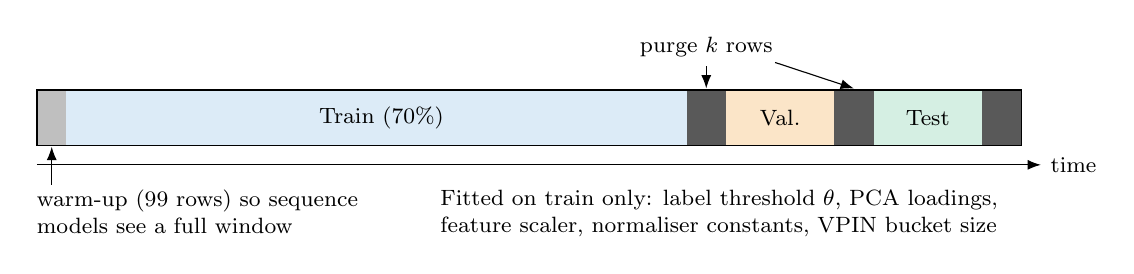
\begin{tikzpicture}[x=0.125cm,y=1cm,font=\footnotesize]
  \fill[boxblue] (0,0) rectangle (70,0.7);
  \fill[boxorange] (70,0) rectangle (85,0.7);
  \fill[boxgreen] (85,0) rectangle (100,0.7);
  \fill[black!65] (66,0) rectangle (70,0.7);
  \fill[black!65] (81,0) rectangle (85,0.7);
  \fill[black!65] (96,0) rectangle (100,0.7);
  \fill[black!25] (0,0) rectangle (3,0.7);
  \draw (0,0) rectangle (100,0.7);
  \node at (35,0.35) {Train (70\%)};
  \node at (75.5,0.35) {Val.};
  \node at (90.5,0.35) {Test};
  \draw[-{Latex}] (0,-0.25) -- (102,-0.25) node[right] {time};
  \node[align=center] at (68,1.25) {purge $k$ rows};
  \draw[-{Latex}] (68,1.0) -- (68,0.72);
  \draw[-{Latex}] (75,1.05) -- (83,0.72);
  \node[align=left,anchor=north west] at (-1,-0.45) {warm-up (99 rows) so sequence\\models see a full window};
  \draw[-{Latex}] (1.5,-0.5) -- (1.5,-0.02);
  \node[align=left,anchor=north west] at (40,-0.45) {Fitted on train only: label threshold $\theta$, PCA loadings,\\ feature scaler, normaliser constants, VPIN bucket size};
\end{tikzpicture}
\caption{Chronological 70/15/15 split with purging. Every model is scored on exactly the same test rows.}\label{fig:split}
\end{figure}

\subsection{Normalisation}
\begin{itemize}
  \item \textbf{Tabular models.} Logistic regression uses features standardised with the training mean and standard deviation. Tree models need no scaling.
  \item \textbf{Deep models} read raw book windows normalised as $(p - P_0)/P_0$ for prices and $\log(1+q/V_0)$ for sizes, where $P_0$ and $V_0$ come from the first 100 training rows. Prices become small relative distances and sizes log-scaled values around 1.
  \item \textbf{BiN} (bilinear normalisation~\cite{tran2021}) is applied inside TLOB; a causal rolling z-score is also implemented.
\end{itemize}

\paragraph{An example of a leak that was caught.} An early version used the relative spread (spread/mid) as a feature. With a fixed tick this is a monotone function of the price \emph{level}, and float32 rounding gave it only two values; LightGBM ranked it as its top feature for the wrong reason, effectively learning where the price was. The spread is now measured in integer ticks.

%% =====================================================================
%%  CHAPTER 4  FEATURES
%% =====================================================================
\chapter{Feature Engineering}

The tabular models receive 27 hand-crafted features per row, all \textbf{causal} (row $t$ uses only rows $\le t$). The deep models receive none of these; they read the raw book and learn their own features.

\section{Feature definitions}

\paragraph{Queue imbalance.} At level 1, $I_t = (q^b_1 - q^a_1)/(q^b_1 + q^a_1) \in [-1,1]$. The same ratio over the first 3, 5 and 10 levels gives the deeper imbalances.

\paragraph{Micro-price deviation.} The size-weighted price $P^{\text{micro}} = (q^b_1 p^a_1 + q^a_1 p^b_1)/(q^b_1+q^a_1)$, so that
\[
P^{\text{micro}}_t - P^{\text{mid}}_t = I_t \cdot \tfrac{S_t}{2}, \qquad S_t = p^a_1 - p^b_1 .
\]

\paragraph{Order flow imbalance (OFI)~\cite{cont2014}.} From one row to the next, the change in bid demand is
\[
\Delta W_t = \begin{cases} q^b_{1,t}, & p^b_{1,t} > p^b_{1,t-1} \\ q^b_{1,t} - q^b_{1,t-1}, & p^b_{1,t} = p^b_{1,t-1} \\ -q^b_{1,t-1}, & p^b_{1,t} < p^b_{1,t-1} \end{cases}
\]
with the ask-side supply change $\Delta V_t$ defined symmetrically, and $\text{OFI}_t = \Delta W_t - \Delta V_t$. Multi-level OFI applies the same formula at each of the 10 levels.

\paragraph{PCA of multi-level OFI.} The 10 per-level OFI values are strongly correlated. Principal component analysis, \textbf{fitted on training rows only}, compresses them to 3 components (on BTC these keep about 60\% of the variance: 36\%, 15\% and 9\%).

\paragraph{VPIN~\cite{easley2012}.} Trades are grouped into buckets of equal volume $V$ (on BTC, the segment's average traded volume per minute in the training period), and
\[
\text{VPIN} = \frac{1}{N}\sum_{\tau=1}^{N} \frac{|V^{B}_\tau - V^{S}_\tau|}{V}, \qquad N = 50 .
\]
Each snapshot gets the VPIN of the last bucket \emph{completed} at or before its timestamp, so it is causal.

\paragraph{Book slopes.} $(p^b_1 - p^b_{10})/\sum_m q^b_m$ and $(p^a_{10} - p^a_1)/\sum_m q^a_m$: price distance per unit of depth; steep means a thin book.

\paragraph{Lags.} Level-1 OFI, imbalance and micro-price deviation 1, 2 and 5 rows earlier give the model the last few seconds of trend.

\begin{table}[H]
\centering\small
\caption{The 27 tabular features}
\label{tab:features}
\begin{tabularx}{\linewidth}{@{}c>{\raggedright\arraybackslash}p{5.2cm}>{\raggedright\arraybackslash}p{2.3cm}X@{}}
\toprule
\textbf{\#} & \textbf{Name} & \textbf{Group} & \textbf{Meaning} \\
\midrule
1 & \code{imbalance\_l1} & L1 snapshot & Bid vs ask size at the best quotes \\
2--4 & \code{imbalance\_l3}, \code{\_l5}, \code{\_l10} & Deeper book / L2--3 & Imbalance over 3, 5, 10 levels \\
5 & \code{spread\_ticks} & L1 snapshot & Spread in integer ticks \\
6 & \code{micro\_deviation} & L1 snapshot & Micro-price minus mid \\
7--8 & \code{slope\_bid}, \code{slope\_ask} & Deeper book & Thickness of each side \\
9 & \code{vpin} & Trade flow & One-sidedness of recent trading \\
10 & \code{ofi\_l1} & L1 snapshot & Net buying pressure at level 1 \\
11--13 & \code{ofi\_pca1}--\code{3} & Deeper book & Multi-level OFI, compressed \\
14--18 & \code{mlofi\_lvl\_1}--\code{5} & L2--3 / deeper & OFI at each of levels 1--5 \\
19--27 & \code{ofi\_lag\_\{1,2,5\}}, \code{imbalance\_lag\_\{1,2,5\}}, \code{micro\_dev\_lag\_\{1,2,5\}} & L1 lags & The level-1 signals 1, 2, 5 rows ago \\
\bottomrule
\end{tabularx}
\end{table}

Two notes on the design. \code{mlofi\_lvl\_1} equals \code{ofi\_l1}, so the 27 columns carry 26 distinct features; this redundancy is harmless for trees. The PCA is fitted on all 10 OFI levels while levels 1--5 are also given raw, so the genuine dimensionality reduction is of levels 6--10.

Figure~\ref{fig:feature_corr} shows the correlation structure. The imbalance features are strongly correlated with each other (0.79--0.93) and the first OFI principal component is close to level-1 OFI (0.91), but the median absolute correlation is only 0.06, so most features carry different information. Tree models are robust to the correlated groups; for logistic regression they are handled by standardisation and the $L_2$ penalty.

\fig{feature_corr}{0.78}{Pearson correlation between the 27 features on the training rows of BTC segment 0.}

\section{Additional features in specific experiments}
\begin{itemize}
  \item \textbf{Order-flow features} (BTC and LOBSTER): limit, market and cancel volume per side at level 1 relative to level-1 depth, their logs over levels 1--5, and the cancel-to-add ratio (14 values).
  \item \textbf{Cross-asset features}: the ETH-USD book features at the latest ETH snapshot at or before each BTC timestamp.
  \item \textbf{FI-2010 history features}: the change of each of the 40 raw book columns over the last 1, 5, 10, 20, 50 and 100 rows (240 features), so tabular models see the same past that DeepLOB sees.
  \item \textbf{Volatility dataset}: realised volatility of the weighted mid price at two levels, spread, depth, imbalance and trade statistics per window, and ``nearest-neighbour'' features averaged over similar windows.
\end{itemize}

%% =====================================================================
%%  CHAPTER 5  METHODOLOGY
%% =====================================================================
\chapter{Machine Learning Methodology}

\section{System overview}

Figure~\ref{fig:pipeline} shows how data flow from the raw book to a profit figure. The same pipeline serves every dataset.

\begin{figure}[H]\centering
\begin{tikzpicture}[font=\footnotesize, >={Latex},
  box/.style={draw, rounded corners=2pt, align=center, execute at begin node={\hyphenpenalty=10000}, minimum height=1.25cm, text width=3.5cm, fill=#1},
  box/.default=boxgrey]
  \node[box] (raw) at (0,0) {Raw data\\BTC/ETH, LOBSTER,\\FI-2010, synthetic};
  \node[box] (conv) at (4.5,0) {Conversion to\\40-column book,\\timestamps, trade tape};
  \node[box] (lab) at (9,0) {Labels (train-only $\theta$),\\purged 70/15/15\\chronological split};
  \node[box=boxblue] (feat) at (4.5,-2.3) {27 causal features\\OFI, MLOFI+PCA,\\VPIN, micro-price, lags};
  \node[box=boxorange] (win) at (9,-2.3) {Raw windows\\$100\times40$, normalised};
  \node[box=boxblue] (tab) at (4.5,-4.6) {Tabular models\\momentum, logistic,\\Random Forest, LightGBM};
  \node[box=boxorange] (deep) at (9,-4.6) {Sequence models\\LSTM, DeepLOB, TLOB\\(Colab A100 GPU)};
  \node[box=boxred] (cpp) at (0,-4.6) {C++ inference\\generated from the\\trained LightGBM};
  \node[box=boxred] (sim) at (0,-7.0) {Execution simulator\\spread, book walk,\\fees, latency, fills};
  \node[box=boxgreen, text width=4.9cm] (eval) at (7.2,-7.0) {Evaluation: macro-F1, AUC, log-loss,\\MCC, IC; bootstrap, McNemar,\\SHAP, ablation};
  \node[box=boxgreen, text width=4.9cm] (pnl) at (3.6,-9.0) {Net P\&L, edge decomposition,\\break-even accuracy, \$ per ms};
  \draw[->] (raw) -- (conv); \draw[->] (conv) -- (lab);
  \draw[->] (lab.south) -- ++(0,-0.25) -| (feat.north);
  \draw[->] (lab) -- (win);
  \draw[->] (feat) -- (tab); \draw[->] (win) -- (deep);
  \draw[->] (tab) -- node[above,font=\scriptsize]{export} (cpp);
  \draw[->] (tab.south) |- ([yshift=0.25cm]eval.north) -- (eval.north);
  \draw[->] (deep.south) |- ([yshift=0.25cm]eval.north);
  \draw[->] (tab.south west) -- node[above left,font=\scriptsize]{signals} (sim.north east);
  \draw[->] (cpp) -- node[left,font=\scriptsize]{latency} (sim);
  \draw[->] (sim.south) |- (pnl.west);
  \draw[->] (eval.south) |- (pnl.east);
\end{tikzpicture}
\caption{End-to-end pipeline: data, features, models, evaluation, execution and latency.}\label{fig:pipeline}
\end{figure}

\section{Learning tasks}

The project uses four kinds of supervised learning problem (Table~\ref{tab:tasks}).

\begin{table}[H]
\centering\small
\caption{Learning tasks}
\label{tab:tasks}
\begin{tabularx}{\linewidth}{@{}>{\raggedright\arraybackslash}p{3.3cm}>{\raggedright\arraybackslash}X>{\raggedright\arraybackslash}p{3.3cm}>{\raggedright\arraybackslash}p{3.0cm}@{}}
\toprule
\textbf{Task} & \textbf{Target} & \textbf{Data} & \textbf{Main metrics} \\
\midrule
3-class classification & Direction of the mid price $k$ rows ahead: UP / FLAT / DOWN & Synthetic, BTC, LOBSTER, FI-2010 & Macro-F1, accuracy, ROC-AUC, log-loss, MCC \\
Regression & Future mid change in bp (also: micro-price change) & BTC, LOBSTER & IC, $R^2$, hit rate \\
Regression & Next 10-minute realised volatility; 60\,s auction price move & Volatility, auction data & RMSPE, MAE \\
Binary classification & Will a resting quote fill, and is the fill ``toxic'' (loses money 30\,s later)? & BTC, LOBSTER & ROC-AUC, markout \\
\bottomrule
\end{tabularx}
\end{table}

\section{The model ladder}

The models form a ladder from no learning to deep learning (Table~\ref{tab:ladder}). A model only counts as good if it beats the simpler ones \emph{on exactly the same test rows}.

\begin{table}[H]
\centering\small
\caption{Model ladder and hyperparameters}
\label{tab:ladder}
\begin{tabularx}{\linewidth}{@{}c>{\raggedright\arraybackslash}p{2.6cm}>{\raggedright\arraybackslash}p{2.6cm}X@{}}
\toprule
\textbf{Tier} & \textbf{Model} & \textbf{Input} & \textbf{Settings} \\
\midrule
0 & Naive momentum, naive flat & past labels & Momentum predicts the last \emph{known} label $y_{t-k}$ (not $y_{t-1}$, which already contains future prices) \\
1 & Logistic regression & 27 features (standardised) & Multinomial, L-BFGS, $C=1$, 1{,}000 iterations \\
2 & Random Forest & 27 features & 100 trees, depth 10, $\ge$10 rows per leaf, balanced subsample weights \\
3 & LightGBM & 27 features & 63 leaves, depth 8, learning rate 0.05, $\le$200 trees, early stopping after 15 rounds on validation loss \\
4 & LSTM & $100\times40$ window & 2 layers $\times$ 64 units, dropout 0.2, 62{,}675 parameters \\
5 & DeepLOB & $100\times40$ window & 3 conv blocks, 2 Inception modules, LSTM(64); 213{,}987 parameters \\
5 & TLOB & $100\times40$ window & BiN, 2 transformer blocks, 4 heads, $d=64$; 88{,}795 parameters \\
\bottomrule
\end{tabularx}
\end{table}

\paragraph{Class weights.} Every learned model weights class $c$ by $n/(3 n_c)$ so that rare UP/DOWN mistakes cost as much as FLAT ones. All models therefore optimise the same objective and macro-F1 is comparable across tiers; the price is lower raw accuracy, because the models predict FLAT less often.

\subsection{Logistic regression}
For each class $c$ the model computes a linear score $z_c = \mathbf{w}_c^\top\mathbf{x} + b_c$ and turns the three scores into probabilities with the softmax $P(y=c\mid\mathbf{x}) = e^{z_c}/\sum_j e^{z_j}$. The weights minimise the weighted cross-entropy plus an $L_2$ penalty. It can only draw linear boundaries, which makes it the reference for ``how much of the signal is linear''.

\subsection{Random Forest}
An ensemble~\cite{breiman2001} of decision trees, each grown on a bootstrap sample of rows and choosing among a random subset of features at each split; the trees vote. Randomisation decorrelates the trees' errors, which reduces variance.

\subsection{Gradient boosting with LightGBM}
Trees are added~\cite{ke2017} one at a time, each fitted to the gradient of the loss with respect to the current prediction:
\[
F_M(\mathbf{x}) = \sum_{m=1}^{M} \eta\, f_m(\mathbf{x}), \qquad f_m \approx \arg\min_f \sum_i L\big(y_i, F_{m-1}(\mathbf{x}_i) + f(\mathbf{x}_i)\big),
\]
with learning rate $\eta=0.05$ and multiclass log-loss $L$ (three trees per round, one per class). LightGBM bins feature values into histograms and grows trees leaf-wise, which makes training fast. Early stopping on the validation loss picks the number of rounds; the BTC model used for the C++ export stopped at 109 rounds (327 trees, 20{,}601 leaves).

\subsection{Recurrent and convolutional networks}

\paragraph{LSTM~\cite{hochreiter1997}.} Reads the window one row at a time, maintaining a gated memory; the last hidden state is classified by a small MLP.

\paragraph{DeepLOB~\cite{zhang2019}.} Treats the $100\times40$ window like an image (Figure~\ref{fig:deeplob}). The first $1\times2$ convolution with stride 2 combines each price with its size; the second combines bid with ask at each level (where something like a micro-price can form); a $1\times10$ convolution combines all levels. Inception modules then look at several time scales in parallel, and an LSTM models the evolution over time.

\begin{figure}[H]\centering
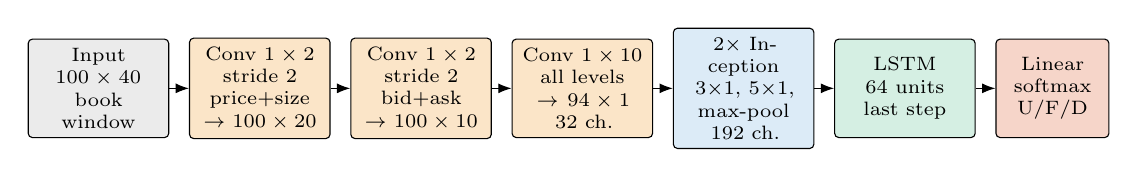
\begin{tikzpicture}[font=\scriptsize, >={Latex},
  l/.style={draw, rounded corners=1.5pt, align=center, minimum height=1.25cm, text width=1.55cm, fill=#1},
  l/.default=boxorange]
  \node[l=boxgrey] (in) {Input\\$100\times40$\\book window};
  \node[l, right=0.25cm of in] (c1) {Conv $1\times2$\\stride 2\\price+size\\$\to 100\times20$};
  \node[l, right=0.25cm of c1] (c2) {Conv $1\times2$\\stride 2\\bid+ask\\$\to 100\times10$};
  \node[l, right=0.25cm of c2] (c3) {Conv $1\times10$\\all levels\\$\to 94\times1$\\32 ch.};
  \node[l=boxblue, right=0.25cm of c3] (inc) {$2\times$ Inception\\$3{\times}1$, $5{\times}1$,\\max-pool\\192 ch.};
  \node[l=boxgreen, right=0.25cm of inc] (lstm) {LSTM\\64 units\\last step};
  \node[l=boxred, right=0.25cm of lstm, text width=1.2cm] (out) {Linear\\softmax\\U/F/D};
  \foreach \a/\b in {in/c1,c1/c2,c2/c3,c3/inc,inc/lstm,lstm/out} \draw[->] (\a) -- (\b);
\end{tikzpicture}
\caption{DeepLOB as implemented (213{,}987 parameters). Each convolution block also has two $4\times1$ temporal convolutions, LeakyReLU and batch normalisation.}\label{fig:deeplob}
\end{figure}

\paragraph{TLOB~\cite{berti2025}.} A transformer~\cite{vaswani2017}: after BiN normalisation and a linear embedding of the 40 columns into 64 dimensions, self-attention lets every time step weigh every other one. Our implementation attends over time steps in both attention layers (the original also attends across features), so it is a simplified TLOB.

\paragraph{Training recipe for all deep models.} Weighted cross-entropy, AdamW (weight decay $10^{-4}$), learning rate $5\times10^{-4}$ (DeepLOB, TLOB) or $10^{-3}$ (LSTM), halved after 2 epochs without validation improvement, gradient clipping at norm 1, batch size 128, at most 10 (synthetic), 8 (BTC) or 15 (FI-2010) epochs, early stopping after 3 epochs with the best weights restored. Training ran in PyTorch with CUDA on Google Colab A100 GPUs.

\subsection{Regression models}
For continuous targets: ridge regression ($\alpha=1$), a LightGBM regressor (500 trees, 63 leaves), and a one-parameter \emph{micro-price rule} $\hat r = \beta\,(P^{\text{micro}} - P^{\text{mid}})$ with $\beta$ fitted by least squares on training rows. The volatility model uses LightGBM with sample weights $1/y^2$, which makes squared error behave like the percentage error being scored; the auction model uses a mean-absolute-error objective.

\section{Validation and leakage control}

\begin{itemize}
  \item \textbf{Purged chronological splits} with train-only fitting of every transform (Section~3.5).
  \item \textbf{Identical test rows.} The sequence windows end exactly on the tabular test rows, with earlier rows as causal context.
  \item \textbf{Purged K-fold cross-validation with embargo} (5 folds, 1\% embargo) in the robustness report.
  \item \textbf{Negative controls.} A model trained on \emph{shuffled} targets must score at chance; across 37 regression cases it averages IC $-0.0005$, and in the robustness report its MCC is $-0.026$.
  \item \textbf{Significance for autocorrelated data.} Neighbouring rows are not independent, so ordinary confidence intervals are too narrow. A \textbf{moving-block bootstrap}~\cite{kunsch1989} resamples 5-minute blocks (300 rows) within each segment, 1{,}000 times, to get a confidence interval for the macro-F1 difference between two models. \textbf{McNemar's test}~\cite{mcnemar1947} compares the rows that only one of two models gets right.
  \item \textbf{Automated tests.} 40 pytest tests check feature formulas, causality (changing the future must not change past features), the purge gap, the momentum baseline, the simulator's fills, and an end-to-end run where a planted signal must be found and the shuffled control must not find it.
\end{itemize}

\section{Evaluation metrics}

\begin{table}[H]
\centering\small
\caption{Metrics used in the report}
\label{tab:metrics}
\begin{tabularx}{\linewidth}{@{}>{\raggedright\arraybackslash}p{3.2cm}>{\raggedright\arraybackslash}X>{\raggedright\arraybackslash}p{3.3cm}@{}}
\toprule
\textbf{Metric} & \textbf{Definition / meaning} & \textbf{Reference values} \\
\midrule
Accuracy & Share of rows predicted correctly & Misleading when FLAT dominates \\
Macro-F1 (main) & Mean over classes of $F_1 = 2PR/(P+R)$; every class counts equally & Random 0.333 (BTC) \\
Balanced accuracy & Mean per-class recall & Random 0.333 \\
ROC-AUC (one-vs-rest) & Probability that a random positive is scored above a random negative, averaged over classes & Random 0.5, perfect 1 \\
Log-loss & $-\frac{1}{n}\sum_i \log \hat p_{i,y_i}$: judges probabilities & Uniform guess $\ln 3 = 1.099$ \\
Brier score & $\frac{1}{n}\sum_i \|\hat{\mathbf p}_i - \mathbf e_{y_i}\|^2$ & Uniform guess 0.667 \\
MCC, Cohen's $\kappa$ & Chance-corrected agreement between prediction and truth & 0 = chance \\
IC & Pearson correlation of forecast with realised move & 0 = no skill \\
$R^2$ (out of sample) & $1 - \text{SSE}/\text{SST}$ & Tiny values are normal at these horizons \\
RMSPE, MAE & Root mean squared percentage error; mean absolute error & Lower is better \\
Hit rate & Share of directional calls with the right sign, on rows that moved & Break-even depends on costs \\
Net P\&L, edge (bp) & Profit after spread, book walking and fees; per round trip in basis points & Must exceed costs \\
Latency (P50, P99) & Median and 99th-percentile time per prediction & Must be well inside the horizon \\
\bottomrule
\end{tabularx}
\end{table}

\section{Execution simulator}

The simulator (\code{src/execution/simulator.py}) turns predictions into trades against the \emph{recorded} book:
\begin{itemize}
  \item \textbf{Taker orders} cross the spread and walk the book level by level, paying the price at each level. Orders larger than the visible depth are extrapolated, partly filled or rejected by a configurable rule.
  \item \textbf{Fees}: 4\bp\ taker and 0\bp\ maker on BTC (Coinbase's top volume tier); 1.5\bp\ taker and a 0.5\bp\ maker rebate on the synthetic book; per-share fees on Nasdaq.
  \item \textbf{Latency} in wall-clock time: an order decided at time $t$ reaches the book at the first snapshot at or after $t+L$, and fills against \emph{that} snapshot.
  \item \textbf{Passive (maker) orders}: since queue position is not observed, three fill rules bracket the truth: \emph{pessimistic} (filled only if the price trades through), \emph{queue} (filled once traded volume at the price exceeds the size ahead), and \emph{optimistic} (front of the queue).
\end{itemize}

\section{Measuring inference speed}

Single-prediction latency is measured as the median (P50) and 99th percentile (P99) wall-clock time to score one row, after warm-up. Python models are timed through their own \code{predict} call on one thread; DeepLOB on a CUDA GPU with batch size 1. A code generator (\code{scripts/lgbm\_to\_cpp.py}) turns the trained LightGBM booster into plain C++ \code{if/else} code; a benchmark checks it against LightGBM on 20{,}000 test rows and times it.

%% =====================================================================
%%  CHAPTER 6  RESULTS: PREDICTION
%% =====================================================================
\chapter{Results: How Well Can the Book Be Predicted?}

\section{Model comparison}

Figure~\ref{fig:model_ladder} and Table~\ref{tab:btc_models} show the model ladder on the synthetic book and on BTC at a 20\,s horizon.

\fig{model_ladder}{1.0}{Test macro-F1 for every model on the synthetic book (left, 5 seeds) and on real BTC (right, 4 segments). Error bars are $\pm1$ standard deviation.}

\begin{table}[H]
\centering\small
\caption{BTC-USD, 20\,s horizon: classification results (mean over 4 segments; $\pm$ std for macro-F1)}
\label{tab:btc_models}
\begin{tabular}{@{}clcccc@{}}
\toprule
\textbf{Tier} & \textbf{Model} & \textbf{Accuracy} & \textbf{Macro-F1} & \textbf{Weighted-F1} & \textbf{Cross-entropy} \\
\midrule
0 & Naive flat & 0.295 & 0.152 & 0.135 & 11.24 \\
0 & Naive momentum & 0.415 & 0.413 $\pm$ 0.021 & 0.415 & 1.440 \\
1 & Logistic regression & 0.463 & 0.448 $\pm$ 0.016 & 0.456 & 1.041 \\
2 & Random Forest & 0.474 & 0.465 $\pm$ 0.017 & 0.471 & 1.029 \\
3 & \textbf{LightGBM} & \textbf{0.476} & \textbf{0.467 $\pm$ 0.021} & \textbf{0.473} & \textbf{1.026} \\
4 & LSTM & 0.448 & 0.397 $\pm$ 0.044 & 0.406 & 1.076 \\
5 & DeepLOB & 0.429 & 0.401 $\pm$ 0.048 & 0.405 & 1.111 \\
5 & TLOB & 0.455 & 0.449 $\pm$ 0.025 & 0.453 & 1.053 \\
\bottomrule
\end{tabular}
\end{table}

\paragraph{Findings.}
\begin{itemize}
  \item \textbf{The signal is real but small.} The best models add about 0.05 macro-F1 over naive momentum and 0.13 over random guessing.
  \item \textbf{Gradient-boosted trees on microstructure features are the best models}, on both synthetic (LightGBM 0.584 $\pm$ 0.012) and real data. Random Forest is almost as good.
  \item \textbf{Deep sequence models do worse here.} DeepLOB and the LSTM trail even momentum on BTC; TLOB is close to logistic regression. With at most 8 epochs they may be under-trained, but they also see only 1\,s snapshots, where hand-made flow features summarise the useful history compactly.
  \item \textbf{Accuracy is not the right metric.} On synthetic data naive flat has the highest accuracy (0.698) and the lowest macro-F1 (0.274).
\end{itemize}

\subsection{Probability-based measures: ROC-AUC, log-loss and calibration}

To report probability-based measures, the tabular models were retrained on each BTC segment with identical settings and their class probabilities kept (\code{report/scripts/btc\_extra\_metrics.py}). Table~\ref{tab:btc_auc} gives the results.

\begin{table}[H]
\centering\scriptsize
\setlength{\tabcolsep}{3.5pt}
\caption{BTC-USD, 20\,s horizon: threshold and probability metrics for the tabular models (mean over 4 segments, $\pm$ std). AUC (U/D) is UP vs DOWN on rows that moved.}
\label{tab:btc_auc}
\begin{tabular}{@{}lccccccccc@{}}
\toprule
\textbf{Model} & \textbf{Acc.} & \textbf{Bal. acc.} & \textbf{Macro-F1} & \textbf{MCC} & \textbf{$\kappa$} & \textbf{ROC-AUC (OvR)} & \textbf{AUC (U/D)} & \textbf{Log-loss} & \textbf{Brier} \\
\midrule
Naive Momentum & 0.415 & 0.413 & 0.413 $\pm$ 0.021 & 0.118 & 0.118 & 0.559 $\pm$ 0.016 & 0.571 & 1.440 & 0.879 \\
Logistic Regression & 0.463 & 0.452 & 0.448 $\pm$ 0.016 & 0.187 & 0.186 & 0.641 $\pm$ 0.017 & 0.710 & 1.041 & 0.626 \\
Random Forest & 0.474 & 0.467 & 0.465 $\pm$ 0.017 & 0.207 & 0.206 & 0.655 $\pm$ 0.019 & 0.717 & 1.029 & 0.619 \\
\textbf{LightGBM} & 0.476 & 0.470 & 0.467 $\pm$ 0.021 & 0.211 & 0.209 & 0.658 $\pm$ 0.022 & 0.717 & 1.026 & 0.617 \\
\midrule
Uniform guess & 0.333 & 0.333 & 0.333 & 0 & 0 & 0.500 & 0.500 & 1.099 & 0.667 \\
\bottomrule
\end{tabular}
\end{table}


\fig{btc_roc_calibration}{1.0}{BTC, 20\,s: ROC curves for UP vs rest and DOWN vs rest (averaged over 4 segments), and a reliability diagram of the predicted probability of the chosen class against how often that class was right.}

\begin{table}[H]
\centering\small
\caption{Macro-F1 and one-vs-rest ROC-AUC by horizon (BTC, mean of 4 segments)}
\label{tab:btc_auc_h}
\begin{tabular}{@{}lcccccc@{}}
\toprule
 & \multicolumn{2}{c}{\textbf{Logistic regression}} & \multicolumn{2}{c}{\textbf{Random Forest}} & \multicolumn{2}{c}{\textbf{LightGBM}} \\
\cmidrule(lr){2-3}\cmidrule(lr){4-5}\cmidrule(lr){6-7}
\textbf{Horizon} & Macro-F1 & AUC & Macro-F1 & AUC & Macro-F1 & AUC \\
\midrule
10\,s & 0.500 & 0.694 & 0.532 & 0.722 & 0.540 & 0.732 \\
20\,s & 0.448 & 0.641 & 0.465 & 0.655 & 0.467 & 0.658 \\
50\,s & 0.382 & 0.578 & 0.396 & 0.585 & 0.395 & 0.584 \\
\bottomrule
\end{tabular}
\end{table}


\paragraph{What the probability metrics add.}
\begin{itemize}
  \item \textbf{ROC-AUC confirms the ranking.} LightGBM has the highest one-vs-rest AUC (0.658), followed closely by Random Forest (0.655), logistic regression (0.641) and momentum (0.559). The ranking is the same as for macro-F1, so it does not depend on the choice of decision threshold.
  \item \textbf{Direction is easier than ``whether it moves''.} On rows whose price did move, LightGBM separates UP from DOWN with AUC 0.717, while FLAT vs rest is only 0.616. Most errors come from deciding whether a move will be large enough, not from its sign.
  \item \textbf{Log-loss and Brier score improve only modestly} on a uniform guess (1.026 vs 1.099, 0.617 vs 0.667): the models are right more often than chance, but rarely sure.
  \item \textbf{The probabilities are well calibrated} (Figure~\ref{fig:btc_roc_calibration}, right): when LightGBM says 64\%, it is right 63\% of the time; only its most confident predictions are slightly over-confident (83\% predicted vs 79\% observed). Calibration matters for trading, because confidence is what decides which signals to trade (Section~7.3).
  \item \textbf{Skill falls with horizon in every measure}: LightGBM's AUC drops from 0.732 at 10\,s to 0.584 at 50\,s (Table~\ref{tab:btc_auc_h}).
  \item MCC (0.211) and Cohen's $\kappa$ (0.209) agree: a real but weak chance-corrected association.
\end{itemize}


\subsection{Statistical significance}

\begin{table}[H]
\centering\small
\caption{Is LightGBM's lead real? Pooled over 4 BTC segments, 20\,s horizon}
\label{tab:signif}
\begin{tabular}{@{}lcccc@{}}
\toprule
\textbf{LightGBM vs} & \textbf{$\Delta$ macro-F1} & \textbf{95\% block-bootstrap CI} & \textbf{Segments better} & \textbf{McNemar $p$} \\
\midrule
Naive momentum & +0.059 & [0.050, 0.068] & 4/4 & $<10^{-4}$ \\
Logistic regression & +0.019 & [0.015, 0.024] & 4/4 & $<10^{-4}$ \\
Random Forest & +0.004 & [0.001, 0.007] & 3/4 & 0.015 \\
DeepLOB & +0.058 & [0.049, 0.068] & 4/4 & $<10^{-4}$ \\
\bottomrule
\end{tabular}
\end{table}

LightGBM is significantly better than all four models, although its lead over Random Forest is tiny. Figure~\ref{fig:btc_confusion} shows where the errors are. FLAT is the hardest class for every model. The tree models spread their mistakes evenly, while DeepLOB leans one way: it calls 41\% of FLAT rows DOWN and recalls DOWN (54\%) much better than UP (42\%).

\fig{btc_confusion}{1.0}{Row-normalised confusion matrices on BTC (20\,s, pooled over segments). F = FLAT, U = UP, D = DOWN.}

\subsection{Simpler models beat deep networks, even in accuracy}\label{sec:simple_vs_deep}

A common expectation is that deep networks reading the raw book are more accurate than simpler models and pay for it only in speed. At the short horizons studied here the opposite holds: the simpler models are \emph{both} more accurate and far faster (Table~\ref{tab:simple_vs_deep}).

\begin{table}[H]
\centering\small
\caption{Best simpler model against the deep networks on the same test rows}
\label{tab:simple_vs_deep}
\footnotesize\setlength{\tabcolsep}{3pt}
\begin{tabular}{@{}llcccl@{}}
\toprule
\textbf{Data, horizon} & \textbf{Metric} & \textbf{Simpler model} & \textbf{DeepLOB} & \textbf{LSTM / TLOB} & \textbf{Winner} \\
\midrule
BTC, 20\,s & Accuracy & \textbf{0.476} (LightGBM) & 0.429 & 0.448 / 0.455 & Simpler \\
BTC, 20\,s & Macro-F1 & \textbf{0.467} (LightGBM) & 0.401 & 0.397 / 0.449 & Simpler \\
Synthetic, 20 ev. & Macro-F1 & \textbf{0.584} (LightGBM) & 0.559 & 0.521 / 0.492 & Simpler \\
FI-2010, $k=10$ & Accuracy (\%) & \textbf{86.1} (logistic + hist.) & 83.1 & -- & Simpler \\
FI-2010, $k=20$ & Accuracy (\%) & \textbf{78.3} (logistic + hist.) & 74.1 & -- & Simpler \\
FI-2010, $k=50$ & Accuracy (\%) & 66.5 (logistic + hist.) & \textbf{78.2} & -- & Deep \\
FI-2010, $k=100$ & Accuracy (\%) & 75.7 (LightGBM + hist.) & \textbf{77.5} & -- & Deep \\
\midrule
\multicolumn{2}{@{}l}{Model size} & 327 trees (LightGBM) & 213{,}987 parameters & 62{,}675 / 88{,}795 & \\
\multicolumn{2}{@{}l}{Training (per BTC segment)} & $\approx$9\,s, laptop CPU & $\approx$18\,min, A100 & & \\
\multicolumn{2}{@{}l}{One prediction} & 10.5\,$\mu$s (C++) & 2.4--5.7\,ms (GPU) & & \\
\bottomrule
\end{tabular}
\end{table}

On BTC, LightGBM's lead over DeepLOB (+0.058 macro-F1) is significant on every segment (Table~\ref{tab:signif}), and DeepLOB and the LSTM score below even naive momentum. Three reasons explain the result:
\begin{itemize}
  \item \textbf{The signal is short-lived and concentrated at the top of the book.} The useful information is level-1 queues and the last few seconds of order flow, which a handful of hand-made features (imbalance, OFI and their lags) capture directly. DeepLOB's own attribution (Section~\ref{sec:drivers}) shows it learns to look at exactly the same things, but it has to discover them from 4{,}000 raw numbers per window.
  \item \textbf{Deep models need more data and training than the signal-to-noise ratio supports.} With 1\,s BTC snapshots and a 20\,s horizon, a network with 214 thousand parameters is easy to overfit to noise; LightGBM with early stopping uses validation data to stop after about a hundred rounds.
  \item \textbf{Seeing history matters more than the architecture.} On FI-2010, giving a linear model the same past 100 rows that DeepLOB sees closes and reverses the gap at short horizons.
\end{itemize}
Deep networks are not useless: on FI-2010 they win clearly at longer horizons ($k=50$--100), where more complex temporal patterns matter. The deep models also had limited tuning (8--15 epochs), so the gap could narrow with more search. The practical conclusion for short-horizon LOB prediction is to start with gradient-boosted trees on microstructure features: they were the most accurate models here, train in seconds, and predict in microseconds.

\section{How fast does the signal decay?}

\fig{signal_decay}{1.0}{Left: BTC skill against horizon. Right: on Nasdaq, the best learned model's macro-F1 minus naive momentum, for large-tick (solid) and small-tick (dashed) stocks.}

\begin{itemize}
  \item \textbf{BTC}: macro-F1 is 0.540 at 10\,s, 0.467 at 20\,s, 0.395 at 50\,s and 0.350 at 100\,s, where LightGBM no longer beats momentum (0.358). The signal lives at the shortest horizons the one-second data allow.
  \item \textbf{Nasdaq large-tick stocks} (INTC, MSFT): learned models beat momentum from 500\,ms to 10\,s, peaking at 1--5\,s (INTC at 5\,s: 0.457 vs 0.344). At 100\,ms nothing is predictable because 99\% of labels are FLAT: a large-tick mid rarely moves that fast.
  \item \textbf{Small-tick stocks} (AMZN, GOOG): the books change so fast that the last move is a strong baseline, and learned models mostly lose to momentum. Order-flow features help them a little (+0.011 macro-F1 on average).
\end{itemize}

\paragraph{Implication for speed.} Useful information lives at horizons of roughly 1--10 seconds and fades after that. Any system that wants to trade on it must act well inside that window, which sets the latency budget used in Chapter~7.

\section{Benchmark against published deep learning: FI-2010}

\fig{fi2010}{0.95}{FI-2010 Setup 2 accuracy (3 seeds). ``+ history'' adds the change of each raw book column over the last 1--100 rows.}

\begin{table}[H]
\centering\small
\caption{FI-2010 Setup 2, test accuracy (\%), mean $\pm$ std over 3 seeds}
\label{tab:fi2010}
\footnotesize\setlength{\tabcolsep}{4pt}
\begin{tabular}{@{}ccccccc@{}}
\toprule
$k$ & \textbf{Naive flat} & \textbf{Logistic} & \textbf{Logistic + hist.} & \textbf{LightGBM + hist.} & \textbf{DeepLOB (ours)} & \textbf{DeepLOB (paper)} \\
\midrule
10 & 70.7 & 70.8 & \textbf{86.1} & 78.0 $\pm$ 0.6 & 83.1 $\pm$ 0.3 & 84.5 \\
20 & 62.1 & 64.1 & \textbf{78.3} & 56.6 $\pm$ 0.0 & 74.1 $\pm$ 0.5 & 74.8 \\
50 & 47.3 & 43.9 & 66.5 & 64.4 $\pm$ 0.0 & \textbf{78.2 $\pm$ 0.2} & 80.5 \\
100 & 34.4 & 40.0 & 60.2 & 75.7 $\pm$ 0.1 & \textbf{77.5 $\pm$ 0.4} & -- \\
\bottomrule
\end{tabular}
\end{table}

\begin{itemize}
  \item \textbf{Our DeepLOB reproduces the paper} to within 0.7--2.3 points, which validates the implementation.
  \item \textbf{At short horizons a linear model with history wins}: 86.1\% vs 83.1\% at $k=10$. DeepLOB's advantage over snapshot features comes mainly from seeing a window of past books, not from its architecture.
  \item \textbf{At long horizons DeepLOB wins clearly} (by 12 points at $k=50$).
  \item \textbf{LightGBM's poor $k=20$ result is distribution shift.} The test days are calmer (62\% FLAT vs 49\% in training). Validation accuracy is 86--88\% for every setting while test accuracy ranges from 55\% to 88\%, so validation data cannot detect the shift. Linear models degrade much less under it.
\end{itemize}

\section{What drives the predictions?}\label{sec:drivers}

\fig{ablation_shap}{1.0}{Left: LightGBM macro-F1 as feature groups are added (BTC, 20\,s). Right: share of TreeSHAP and split-gain importance by feature group.}

\begin{itemize}
  \item \textbf{Ablation.} The level-1 snapshot alone (4 features) reaches 0.436. Adding the 9 lags of level-1 signals gives the largest single gain (+0.024); everything deeper adds less than 0.01.
  \item \textbf{TreeSHAP} (exact, from LightGBM's \code{pred\_contrib}, on 20{,}000 test rows per segment): deeper-book shape 39\%, level-1 lags 35\%, level-1 snapshot 14\%, VPIN 7\%, levels 2--3 5\%. Gain importance under-weights the lags (25\%), showing why gain is not a reliable attribution.
  \item \textbf{DeepLOB} (gradient $\times$ input on 2{,}000 windows per segment) also concentrates on the top of the book and on recent history: level 1 counts twice as much as any deeper level, and 57\% of the weight falls on the most recent 10 of its 100 snapshots (Figure~\ref{fig:deeplob_attribution}). The deep network, without hand-made features, ends up using the same information as LightGBM.
  \item \textbf{Cross-asset.} Adding ETH-USD book features improves BTC macro-F1 by +0.016 at 10\,s, +0.012 at 20\,s and +0.007 at 50\,s, on all 4 segments; the fading gain fits ETH leading BTC by a few seconds.
\end{itemize}

\fig{deeplob_attribution}{0.85}{DeepLOB gradient $\times$ input attribution on BTC (mean of 4 segments). *The price/size split is partly a scaling effect, because gradient $\times$ input grows with the input's magnitude.}

\section{Regression results}\label{sec:regression}

\subsection{The micro-price as predictor and as target}

\fig{microprice}{1.0}{Left: slope $\beta$ of the future mid change on today's micro-price gap. Right: information coefficient (IC) of four forecasts with the realised future mid change.}

\begin{table}[H]
\centering\small
\caption{IC with the future mid change (test period)}
\label{tab:micro}
\footnotesize\setlength{\tabcolsep}{4pt}
\begin{tabular}{@{}lcccc@{}}
\toprule
 & \textbf{Large tick 5\,s} & \textbf{Large tick 10\,s} & \textbf{Small tick 1\,s} & \textbf{BTC 10\,s} \\
\midrule
Micro-price rule ($\beta\times$ gap, 1 parameter) & \textbf{0.290} & \textbf{0.278} & 0.062 & 0.024 \\
Momentum (past return) & 0.037 & 0.012 & 0.042 & 0.074 \\
Ridge regression & -- & -- & -- & 0.241 \\
LightGBM, trained on mid change & 0.209 & 0.170 & \textbf{0.155} & \textbf{0.263} \\
LightGBM, trained on micro-price change & 0.080 & 0.009 & $-$0.007 & 0.260 \\
Shuffled-target control & $-$0.003 & 0.005 & $-$0.003 & 0.002 \\
\bottomrule
\end{tabular}
\end{table}

\begin{itemize}
  \item On large-tick stocks the mid closes the gap to the micro-price within about 10\,s ($\beta=0.93$), and the \textbf{one-parameter rule matches or beats LightGBM} from 5\,s on, getting the sign right 64--82\% of the time. This matters for speed: the rule costs a handful of arithmetic operations.
  \item As a \emph{training target}, the micro-price is worse than the mid in 21 of 37 cases (block-bootstrap CIs) and never better.
  \item On BTC, LightGBM regression reaches IC 0.263 and out-of-sample $R^2$ 0.067 at 10\,s; ridge regression reaches 0.241 and 0.057.
\end{itemize}

\subsection{Volatility regression and the cost of leakage}

Volatility is far more predictable than direction. On the realised-volatility data, LightGBM cuts the naive error (current volatility) by about 30\% (RMSPE 0.235 vs 0.337). The best published solution added ``nearest-neighbour'' features averaged over similar time windows, \emph{including future ones}. Restricting the neighbours to the past keeps only about 59\% of their gain (Figure~\ref{fig:optiver_leakage}), and shuffled K-fold cross-validation makes a plain model look as good as the leaky one. The design of the validation changes the conclusion.

\fig{optiver_leakage}{0.75}{Realised-volatility regression on 4 forward-in-time folds (RMSPE, lower is better).}

On the closing-auction data (481 days, train on the first 400), LightGBM improves MAE over predicting zero by 2.4\% (5.848 vs 5.994), and retraining every 12 days helps only marginally under the drift.

\section{Classifying toxic fills}

For market making, a LightGBM classifier predicts whether a resting quote will fill and whether the fill will lose money 30\,s later (a ``toxic'' fill). Given a fill, it separates toxic from good fills with ROC-AUC 0.55--0.58 on BTC and 0.39--0.53 on Nasdaq: adverse selection is only weakly predictable. VPIN does not sort fills by toxicity, and across 54 regime cells (VPIN, spread and volatility terciles) predictability is highest in \emph{calm} markets (macro-F1 0.483 in low volatility vs 0.443 in high), not toxic ones.

%% =====================================================================
%%  CHAPTER 7  ACCURACY, SPEED AND PROFIT
%% =====================================================================
\chapter{From Prediction to Profit: Accuracy, Speed and Cost}

\section{A simple model of the trading edge}

For one round trip (enter, hold for horizon $h$, exit) with predicted direction $s=\pm1$ and mid change $\Delta m$, the expected net edge is
\[
\text{net edge} = \underbrace{E[s\,\Delta m_{t\to t+h}]}_{\text{accuracy}} - \underbrace{\big(E[s\,\Delta m_{t\to t+h}] - E[s\,\Delta m_{t+L\to t+L+h}]\big)}_{\text{latency } L} - \underbrace{c_{\text{cross}}}_{\text{spread, depth}} - \underbrace{2f}_{\text{fees}} .
\]
The ML model controls the first term, the system's speed the second, and the market and exchange the last two. If moves have average size $m$ and the model is right with probability $p$, the first term is about $(2p-1)m$, so breaking even after a total round-trip cost $C$ needs a hit rate of
\[
\boxed{\,p^* = \tfrac12 + \frac{C}{2m}\,}
\]
Better models raise $p$, faster systems shrink $C$, and if $C > m$ no model can win at all.

\section{BTC: the edge exists, but costs remove it}

\fig{pnl_regimes}{1.0}{Net P\&L of the same predictions under three execution assumptions: at the mid with no costs (as many papers report), as an aggressive taker, and as a passive maker. Mean $\pm$ std over seeds/segments.}

On BTC, LightGBM's test signals earn \$8{,}055 $\pm$ 988 per test window if trades happen at the mid with no costs, but lose \$36{,}394 $\pm$ 7{,}271 as an aggressive taker with 1\,s latency, because fees alone (\$37{,}631) are 4.7 times the cost-free profit. On the synthetic book, crossing the spread and paying fees removes 75\% of LightGBM's cost-free P\&L and 94\% of DeepLOB's. DeepLOB's signals flip more often, so it trades more and pays more friction.

\section{Where the edge goes, and how accuracy changes it}

Each BTC round trip was split into the edge at the decision mid, the cost of reacting one snapshot (1\,s) later, and the cost of crossing the spread and walking the book.

\fig{edge_waterfall}{0.8}{Decomposition of the average round trip for the most confident 2\% of LightGBM signals on BTC (20\,s hold).}

\begin{table}[H]
\centering\small
\caption{BTC round-trip decomposition by confidence (LightGBM, 20\,s hold, bp per round trip)}
\label{tab:edge}
\footnotesize\setlength{\tabcolsep}{3.5pt}
\begin{tabular}{@{}lccccccc@{}}
\toprule
\textbf{Signals traded} & \textbf{Trades} & \textbf{Edge} & \textbf{1\,s delay} & \textbf{Crossing} & \textbf{Gross} & \textbf{Hit rate} & \textbf{Break-even, 0/1/4\bp\ fee} \\
\midrule
All & 6{,}359 & 1.01 & $-$0.27 & $-$0.73 & 0.01 & 60.7\% & 63\% / 90\% / $>$100\% \\
Top 10\% & 3{,}776 & 1.97 & $-$0.65 & $-$0.89 & 0.43 & 68.9\% & 68\% / 92\% / $>$100\% \\
Top 2\% & 1{,}590 & 2.23 & $-$0.75 & $-$1.01 & 0.47 & 71.8\% & 70\% / 94\% / $>$100\% \\
\bottomrule
\end{tabular}
\end{table}

\fig{hit_rate_breakeven}{1.0}{Left: share of UP/DOWN calls with the right sign, on rows labelled UP or DOWN, as the models keep only their most confident predictions (retrained tabular models, 4 segments, $\pm$ std). Right: the hit rate needed to break even, $p^*$, against round-trip cost, with LightGBM's achieved hit rates.}

The left panel of Figure~\ref{fig:hit_rate_breakeven} shows that confidence filtering works for all three tabular models: on rows whose label is UP or DOWN, the share of directional calls with the right sign rises from about 69\% when every row is traded to 86--87\% for the most confident 2\%. (These hit rates are higher than in Table~\ref{tab:edge} because there only rows with a label beyond the threshold count, whereas the table scores every traded mid move, however small.)

\paragraph{Four findings.}
\begin{enumerate}
  \item \textbf{Better accuracy doubles the edge.} Trading only confident signals raises the hit rate from 61\% to 72\% and the edge from 1.0 to 2.2\bp.
  \item \textbf{Better signals are more sensitive to latency.} A 1\,s delay costs 0.27\bp\ on all signals but 0.75\bp\ on the top 2\%. The most confident signals predict the moves that come soonest, so waiting hurts them most.
  \item \textbf{Without fees, confident signals clear the bar} (72\% achieved vs 70\% needed). With a 1\bp\ fee they would need 94\%.
  \item \textbf{At the real 4\bp\ taker fee, no accuracy is enough.} The average absolute 20\,s move is about 4.3\bp, so even a perfect forecast earns less than the 8\bp\ round-trip fee: $C>m$, so $p^*>1$.
\end{enumerate}

\section{How fast is each model?}

\begin{table}[H]
\centering\small
\caption{Time to make one prediction}
\label{tab:latency}
\begin{tabularx}{\linewidth}{@{}>{\raggedright\arraybackslash}p{4.6cm}cc>{\raggedright\arraybackslash}X@{}}
\toprule
\textbf{Model / step} & \textbf{P50} & \textbf{P99} & \textbf{Notes} \\
\midrule
Logistic regression (Python) & 137\,$\mu$s & 264\,$\mu$s & Batch: 0.19\,$\mu$s/row; fit 2\,s \\
Random Forest, 100 trees (Python) & 42.57\,ms & 47.54\,ms & Batch: 1.56\,$\mu$s/row; fit 15\,s \\
LightGBM booster (Python, 1 thread) & 109\,$\mu$s & 217\,$\mu$s & Batch: 40.70\,$\mu$s/row; fit 9\,s \\

LightGBM compiled to C++ (327 trees) & 10.5\,$\mu$s & 17.9\,$\mu$s & Bit-identical to Python (max diff 0, 100\% agreement) \\
Features + 50-tree ensemble + order, C++ & 1.9\,$\mu$s & 6.3\,$\mu$s & $\approx$399{,}000 snapshots/s \\
DeepLOB, GPU, batch 1 & 2.4--5.7\,ms & -- & Synthetic / BTC \\
Micro-price rule & a few ns & -- & A few arithmetic operations \\
\midrule
BTC data interval & 1\,s & & Fastest possible reaction in this data \\
Signal horizon (Nasdaq peak) & 1--5\,s & & From Section 6.2 \\
\bottomrule
\end{tabularx}
\end{table}

\fig{speed_vs_accuracy}{0.85}{Accuracy against inference speed on BTC. The most accurate model (LightGBM) is also one of the fastest, and compiling it to C++ makes it 230--540 times faster than DeepLOB on a GPU without changing a single prediction. Random Forest is accurate but slow from Python (100 trees, thread start-up on every call).}

The accuracy--speed trade-off that is often assumed (``deep models are more accurate but slower'') does not hold at these horizons: the tree model is both more accurate and orders of magnitude faster.

\section{Converting latency into profit}

To measure the value of speed directly, the synthetic book (events about 10\,ms apart, horizon 20 events $\approx$ 200\,ms) was traded as an aggressive taker with extra latency added to each order.

\fig{latency_pnl}{1.0}{Net P\&L against added latency. Left: synthetic large-tick book (5 seeds; shaded band $\pm1$ standard error). Right: BTC (4 segments), where latency is in whole seconds.}

\begin{table}[H]
\centering\small
\caption{Synthetic latency sweep: net P\&L per test window (\$, mean of 5 seeds)}
\label{tab:sweep}
\begin{tabular}{@{}lcccccc@{}}
\toprule
\textbf{Added latency} & 0\,ms & 1\,ms & 10\,ms & 25\,ms & 50\,ms & 100\,ms \\
\midrule
LightGBM & 508 & 457 & 427 & 369 & 290 & 119 \\
DeepLOB & 155 & 104 & 71 & 14 & $-$76 & $-$247 \\
\bottomrule
\end{tabular}
\end{table}

\begin{enumerate}
  \item \textbf{Both models lose about the same per millisecond}: \$3.4 (LightGBM) and \$3.6 (DeepLOB) per ms on average.
  \item \textbf{DeepLOB's slower inference costs little.} Its extra $\approx$2.3\,ms of GPU inference costs about \$10, while LightGBM's lead at zero latency, which comes purely from better signals, is about \$350. At these speeds, choosing the more accurate model is worth \textbf{about 35 times more} than choosing the faster one.
  \item \textbf{Accuracy buys latency budget.} DeepLOB's smaller edge is gone by about 30\,ms, a seventh of the horizon. LightGBM's is still positive at 100\,ms, half the horizon (extrapolated break-even $\approx$134\,ms). A more accurate model tolerates a slower system.
  \item \textbf{On BTC as a taker, latency barely matters.} Going from 1\,s to 0\,s improves P\&L by only about 5\% ($-$\$36.4k to $-$\$34.5k), and even 30\,s of delay only moves it to $-$\$41.0k, because fees dominate.
\end{enumerate}

\section{Passive trading: when speed is the edge}

A market maker posts resting orders and earns the spread instead of paying it, but its orders tend to fill just before the price moves against them (adverse selection).

\begin{itemize}
  \item \textbf{BTC:} there is no spread to earn (0.0017\bp). Naive two-sided quoting loses about \$10{,}400 a day. Quoting only when the toxic-fill model predicts a positive value cuts losses by 86\% or more, but breaks even only under optimistic fills.
  \item \textbf{Nasdaq large-tick stocks:} the result depends on queue position, which is a pure speed race. Measured 30\,s after the fill, a fill at the front of the queue earns +1.24\bp\ (INTC) and +0.70\bp\ (MSFT); a fill at the back loses 2.22\bp\ and 1.78\bp. With about 13{,}000 shares already queued, a new order is almost always at the back.
\end{itemize}
Here prediction helps decide \emph{when} to quote, but latency, not accuracy, decides whether quoting pays.

\section{The balancing rule}

For a strategy with signal horizon $h$, system latency $L$ and round-trip cost $C$:
\begin{enumerate}
  \item \textbf{Check feasibility first.} Is the typical move $m$ over horizon $h$ clearly larger than $C$? If not, no model or system will work; change the instrument, horizon or execution style.
  \item \textbf{Choose the model by accuracy at that horizon}, among models whose inference fits well inside $h$. At a few seconds every model fits; near 100\,ms only microsecond models fit; at longer horizons deep models become affordable and, on FI-2010, more accurate.
  \item \textbf{Spend on latency in proportion to how fast the signal decays.} Keep $L$ a small fraction of $h$, smaller for better signals because their edge is concentrated in the first moments.
  \item \textbf{For passive execution,} queue position (speed) dominates; prediction is the filter.
\end{enumerate}

%% =====================================================================
%%  CHAPTER 8  DISCUSSION
%% =====================================================================
\chapter{Discussion, Limitations and Future Work}

\section{What the results mean for machine learning on LOB data}
\begin{itemize}
  \item \textbf{Feature engineering still beats raw-input deep learning at short horizons} on these data. Domain features (OFI, imbalance, lags) encode exactly the information that DeepLOB's attribution shows it learns to look for, but with far less data and compute.
  \item \textbf{The input matters more than the architecture.} On FI-2010, giving a linear model the same history DeepLOB sees closes and reverses the gap at short horizons.
  \item \textbf{Validation design changes the answer.} Shuffled cross-validation, full-sample normalisation, a relative-spread feature and look-ahead neighbours each produced convincing but false improvements during this project.
  \item \textbf{Classification metrics are not economic metrics.} A 0.05 macro-F1 gain is statistically certain and economically worthless at a 4\bp\ fee, but valuable with a 0\bp\ fee.
\end{itemize}

\section{Limitations}
\begin{itemize}
  \item \textbf{Small real samples.} BTC covers 12 days from one exchange; LOBSTER is one day per stock with the test period in the last hour. LOBSTER numbers are a case study.
  \item \textbf{Coarse BTC data.} With 1\,s snapshots, the ``1\,s delay'' is the data's resolution, not a real system latency; sub-second effects on BTC are invisible.
  \item \textbf{Unobserved queue position}, so passive fills are reported as bounds.
  \item \textbf{No persistent price impact}: our orders walk the snapshot they arrive on but do not deplete later snapshots.
  \item \textbf{Synthetic latency sweep}: the generator plants the signal, so dollar-per-millisecond figures show the mechanism, not real-market magnitudes; test windows are short ($\approx$90\,s per seed).
  \item \textbf{Limited tuning of deep models} (8--15 epochs, little hyperparameter search) and a simplified TLOB.
  \item \textbf{Timing}: the C++ model was timed on a busy machine (an upper bound) and covers inference only, not network or feed handling.
  \item \textbf{Many comparisons} in the regime study (54 cells); only patterns consistent across segments and models are reported.
\end{itemize}

\section{Future work}
\begin{itemize}
  \item Passive execution on large-tick stocks with a queue-position model, using full LOBSTER data over many days.
  \item Deep models on sub-second Nasdaq data, to test whether ``deep wins at long horizons'' holds outside FI-2010.
  \item A volatility-normalised history feature set to test the FI-2010 distribution-shift explanation, and online/retrained models for non-stationarity.
  \item Wire-to-order latency: an order-book engine, a feed parser and kernel-bypass networking around the generated C++ model.
\end{itemize}

%% =====================================================================
%%  CHAPTER 9  CONCLUSION
%% =====================================================================
\chapter{Conclusion}

This project used limit order book data, a much richer input than ordinary price bars, to study what machine learning can predict about the next few seconds of a market, and whether that prediction is worth anything once it has to be traded.

\section{Summary of results}
\begin{itemize}
  \item \textbf{Data.} Six datasets (1.03 million BTC and ETH snapshots, every Nasdaq order event for five stocks, FI-2010, two regression datasets and a synthetic book) were converted to a common 40-column format, labelled with train-only thresholds and split chronologically with purging.
  \item \textbf{Prediction.} The book is significantly but modestly predictive. On BTC at 20\,s, LightGBM reaches macro-F1 0.467 (random 0.333, momentum 0.413) and beats every other model with bootstrap CIs excluding zero. On large-tick stocks the signal is stronger and peaks at 1--5\,s.
  \item \textbf{Models.} Simpler models beat deep networks at short horizons, in accuracy as well as speed: on BTC at 20\,s LightGBM is more accurate than DeepLOB (0.476 vs 0.429 accuracy, 0.467 vs 0.401 macro-F1), the LSTM and TLOB, and on FI-2010 logistic regression with book history beats DeepLOB at $k=10$--20. DeepLOB, reproduced to within 2.3 points of the paper, wins only at longer horizons on FI-2010. A one-parameter micro-price rule matches LightGBM on large-tick stocks.
  \item \textbf{What the models use.} The top of the book and its last few seconds of history, for both LightGBM (SHAP, ablation) and DeepLOB (gradient attribution).
  \item \textbf{Speed and profit.} Accuracy, speed and cost interact. On the synthetic book accuracy is worth 35 times more than inference speed, and a more accurate model tolerates more latency. Better signals decay faster, so they need faster execution. On BTC the 8\bp\ taker round trip exceeds the typical 4.3\bp\ move, so no model can profit; costs set the bar.
  \item \textbf{Engineering.} The trained LightGBM was compiled into C++ with identical output and 10.5\,$\mu$s median latency, 230--540 times faster than DeepLOB on a GPU.
\end{itemize}

The practical recipe that falls out is: pick a market and execution style where the typical move exceeds the cost; pick the most accurate model whose inference fits well inside the signal's horizon, which at short horizons is a simple model compiled to fast code; and invest in speed in proportion to how concentrated the signal is in its first moments.

%% =====================================================================
%%  REFERENCES
%% =====================================================================
\renewcommand{\bibname}{References}
\cleardoublepage\phantomsection\addcontentsline{toc}{chapter}{References}
\begin{thebibliography}{99}
\bibitem{cont2014} R.~Cont, A.~Kukanov and S.~Stoikov, ``The price impact of order book events,'' \emph{Journal of Financial Econometrics}, vol.~12, no.~1, pp.~47--88, 2014.
\bibitem{easley2012} D.~Easley, M.~M.~L\'opez de Prado and M.~O'Hara, ``Flow toxicity and liquidity in a high-frequency world,'' \emph{Review of Financial Studies}, vol.~25, no.~5, pp.~1457--1493, 2012.
\bibitem{stoikov2018} S.~Stoikov, ``The micro-price: a high-frequency estimator of future prices,'' \emph{Quantitative Finance}, vol.~18, no.~12, pp.~1959--1966, 2018.
\bibitem{zhang2019} Z.~Zhang, S.~Zohren and S.~Roberts, ``DeepLOB: Deep convolutional neural networks for limit order books,'' \emph{IEEE Transactions on Signal Processing}, vol.~67, no.~11, pp.~3001--3012, 2019.
\bibitem{ntakaris2018} A.~Ntakaris, M.~Magris, J.~Kanniainen, M.~Gabbouj and A.~Iosifidis, ``Benchmark dataset for mid-price forecasting of limit order book data with machine learning methods,'' \emph{Journal of Forecasting}, vol.~37, no.~8, pp.~852--866, 2018.
\bibitem{tran2021} D.~T.~Tran, J.~Kanniainen, M.~Gabbouj and A.~Iosifidis, ``Data normalization for bilinear structures in high-frequency financial time-series,'' in \emph{Proc. ICPR 2020}, 2021.
\bibitem{berti2025} L.~Berti and G.~Kasneci, ``TLOB: A novel transformer model with dual attention for price trend prediction with limit order book data,'' arXiv:2502.15757, 2025.
\bibitem{ke2017} G.~Ke, Q.~Meng, T.~Finley, T.~Wang, W.~Chen, W.~Ma, Q.~Ye and T.-Y.~Liu, ``LightGBM: A highly efficient gradient boosting decision tree,'' in \emph{Advances in Neural Information Processing Systems 30}, 2017.
\bibitem{lopez2018} M.~L\'opez de Prado, \emph{Advances in Financial Machine Learning}. Hoboken, NJ: Wiley, 2018.
\bibitem{lundberg2017} S.~M.~Lundberg and S.-I.~Lee, ``A unified approach to interpreting model predictions,'' in \emph{Advances in Neural Information Processing Systems 30}, 2017.
\bibitem{breiman2001} L.~Breiman, ``Random forests,'' \emph{Machine Learning}, vol.~45, no.~1, pp.~5--32, 2001.
\bibitem{hochreiter1997} S.~Hochreiter and J.~Schmidhuber, ``Long short-term memory,'' \emph{Neural Computation}, vol.~9, no.~8, pp.~1735--1780, 1997.
\bibitem{vaswani2017} A.~Vaswani et al., ``Attention is all you need,'' in \emph{Advances in Neural Information Processing Systems 30}, 2017.
\bibitem{huang2015} R.~Huang and T.~Polak, ``LOBSTER: Limit order book reconstruction system,'' SSRN 1977207, 2011. [Online]. Available: \url{https://lobsterdata.com}
\bibitem{kunsch1989} H.~R.~K\"unsch, ``The jackknife and the bootstrap for general stationary observations,'' \emph{Annals of Statistics}, vol.~17, no.~3, pp.~1217--1241, 1989.
\bibitem{mcnemar1947} Q.~McNemar, ``Note on the sampling error of the difference between correlated proportions or percentages,'' \emph{Psychometrika}, vol.~12, no.~2, pp.~153--157, 1947.
\bibitem{repo} Project repository: code, experiment artefacts, \code{README.md}, \code{submission/PROJECT\_REPORT.md} and \code{docs/learn/}.
\end{thebibliography}

\end{document}
